\chapter{Алгоритм синтаксического анализа регулярной аппроксимации} \label{AlgoDescr}

В данной главе формально описана задача синтаксического анализа динамически формируемых выражений, а так же изложен алгоритм её решения. Также сформулированы и доказаны утверждения о корректности данного алгоритма.

\section{Постановка задачи}

Анализируемая программа $\mathcal{P}$ является генератором выражений и таким образом задаёт некоторый язык $L_1$. Предположим, что $\mathcal{P}$ взаимодействует с базой данных с помощью динамически формируемых выражений. В этом случае мы говорим, что $\mathcal{P}$ использует динамический SQL, подразумевая, что программой генерируются выражения на языке SQL. Однако это не совсем корректно, так как программа может, например, содержать ошибку и некоторые из построенных ей выражений не будут корректными SQL-выражениями. Кроме того, программа $\mathcal{P}$ может генерировать не все возможные выражения на SQL. Таким образом, в этом случае $L_1\neq$~SQL.

С другой стороны, может быть задан эталонный язык $L_2$ --- язык, которому должны принадлежать все выражения генерируемые программой $\mathcal{P}$. Как правило $L_2$ описывается с помощью контекстно-свободной грамматики. Например, это может быть грамматика конкретного диалекта SQL, взятая из документации.

В результате мы имеем описание двух языков, и задача проверки корректности выражений, генерируемых $\mathcal{P}$, может быть сформулирована как проверка вложенности языка $L_1$ в язык $L_2$. Однако в рамках данной работы нас интересует не просто вложенность языков, а построение деревьев вывода. Как уже говорилось, язык $L_2$ может быть задан с помощью грамматики. Пусть задана грамматика $G$, такая, что $L_2 = L(G)$, тогда задача синтаксического анализа динамически формируемых выражений может быть поставлена следующим образом: для всех цепочек $\omega \in L_1$, выводимых в грамматике $G$, построить соответствующие деревья вывода.

Отметим, что решение изложенных выше вопросов в общем виде возможно не всегда. Трудности могут быть связаны прежде всего с классами рассматриваемых языков. Эталонный язык $L_2$, скорее всего, является некоторым языком программирования и принадлежит к классу контекстно-свободных языков (хотя могут быть и исключения). Генерируемый язык $L_1$, вообще говоря, не обязан быть даже контекстно-зависимым. Так как программа-генератор реализована на тьюринг-полном языке, то $L_1$ в общем случае может быть рекурсивно-перечислимым. Из практических соображений хочется думать, что $L_1$ всё же является подмножеством некоторого языка программирования и может быть достаточно хорошо приближен некоторым контекстно-свободным языком. Однако проверка включения двух контекстно-свободных языков не разрешима в общем случае~\cite{LangIncusion}. При этом разрешима в общем случае проверка включения регулярного языка в однозначный контекстно-свободный~\cite{LangIncusion}. В однозначные контекстно-свободные языки попадают такие практически значимые классы, как LR(k) и LL(k), что позволяет использовать в качестве $L_2$ практически значимые языки. При этом для $L_1$ необходимо строить регулярное приближение $L_R$.

Чтобы обеспечить надёжность анализа строковых выражений, необходима аппроксимация сверху, то есть должно выполняться включение $L_1 \subseteq L_R$. Это необходимо для того, чтобы не потерять информацию об анализируемом языке. Например, при работе со встроенным SQL безопаснее считать таблицу используемой, чем удалить её как неиспользуемую, если она на самом деле использовалась. При этом необходимо следить за точностью такой аппроксимации, чтобы избегать слишком большого количества ошибок. В работе~\cite{RegOverApprox} показано, как можно строить достаточно точную регулярную аппроксимацию сверху с учётом строковых операций и циклов.

Таким образом, далее мы будем предполагать, что язык $L_2$ является однозначным контекстно-свободным и задан некоторой грамматикой $G$, а для языка $L_1$ строится регулярный язык $L_R$ такой, что $L_1 \subseteq L_R$ и мы работает далее с $L_R$. При этом основной нашей задачей является построение деревьев разбора для всех цепочек из $L_R$, корректных относительно грамматики $G$. Однако $L_R$ может быть бесконечным языком и, следовательно, содержать бесконечное множество корректных цепочек. По этой причине явное построение всех деревьев разбора не представляется возможным. Решением, возможно, будет являться структура, которая при конечном объёме будет хранить бесконечное количество деревьев. При этом деревья должны однозначно извлекаться из этой структуры. То есть из построенной структуры можно получить только те и только те деревья, которые соответствуют разбору какой-либо корректной цепочки из $L_R$ языка в эталонной грамматике $G$.

Регулярный язык $L_R$ может быть представлен в виде конечного автомата. Заметим, что аппроксимация, построенная непосредственно по исходному коду, будет являться конечным автоматом $M_1=(Q_1,\Sigma_1,\delta_1,q_{0_1},q_{f_1})$ над алфавитом символов, что не очень удобно для проведения синтаксического анализа, так как грамматика $G = \langle T, N, P, S \rangle$ задана, скорее всего, над алфавитом токенов и $\Sigma_1 \nsubseteq T$. Чтобы устранить эту проблему, можно воспользоваться конечным преобразователем, который предназначен для трансформации языков. Таким образом, можно получить конечный автомат $M_2=(Q_2,\Sigma_2,\delta_2,q_{0_2},q_{f_2})$ такой, что $\Sigma_2 \subseteq T$. Преобразование конечного автомата над алфавитом символов в конечный автомат над алфавитом токенов называется лексическим анализом регулярной аппроксимации или встроенного языка.

Заметим так же, что без потери общности можно считать, что $M_2$ является детерминированным конечным автоматом без $\varepsilon$-переходов, так как любой конечный автомат можно преобразовать к эквивалентному детерминированному без  $\varepsilon$-переходов.

Таким образом, решаемая в данной работе задача синтаксического анализа динамически формируемых выражений будет формулироваться следующим образом. \textit{ Для данной однозначной контекстно-свободной грамматики $G = \langle T, N, P, S \rangle$ и детерминированного конечного автомата без $\varepsilon$-переходов $M=(Q,\Sigma,\delta,q_0,q_f)$ такого, что $\Sigma \subseteq T$, необходимо построить конечную структуру данных $F$, содержащую деревья вывода в $G$ всех цепочек $\omega \in L(M)$, корректных относительно грамматики $G$, и не содержащую других деревьев. } Иными словами, необходимо построить алгоритм $\mathbb{P}$ такой, что
    $$(\forall \omega \in L(M)) (\omega \in L(G) \Rightarrow (\exists t \in \mathbb{P}(L(M),G))AST(t, \omega, G))$$
    $$\land (\forall t \in \mathbb{P}(L(M),G))(\exists \omega \in L(M))AST(t,\omega,G).$$ 
    Здесь $AST(t,\omega,G)$ --- это предикат, который истинен, если $t$ является деревом вывода $\omega$ в грамматике $G$.


Так как $\mathbb{P}$ игнорирует ошибки, то будем называть его алгоритмом \textit{ослабленного} (relaxed) синтаксического анализа регулярной аппроксимации динамически формируемого выражения.


\section{Описание алгоритма ослабленного синтаксического анализа регулярной аппроксимации}\label{AlgoDescr}

Алгоритм принимает на вход эталонную однозначную контекстно-свободную грамматику $G=\langle T, N, P, S \rangle$ над алфавитом терминальных символов $T$ и детерминированный конечный автомат $(Q,\Sigma,\delta,q_0,q_f)$, имеющий одно стартовое состояние $q_0$, одно конечное состояние $q_f$, и не содержит $\varepsilon$-переходов, где $\Sigma \subseteq T$~--- алфавит входных символов, $Q$~--- множество состояний, $\delta$~--- отношение перехода. По описанию  грамматики генерируются управляющие RNGLR-таблицы и некоторая вспомогательная информация (называемая $parserSource$ в псевдокоде, см. листинг~\ref{parsing}). 

\begin{listing}[!ht]
\hrule

\begin{algorithmic}[1]
\caption{Алгоритм ослабленного синтаксического анализа регулярной аппроксимации динамически формируемого выражения}
\label{parsing}
\Function{parse}{$grammar, automaton$}
  \State{$inputGraph \gets$ construct inner graph representation of $automaton$}
  \State{$parserSource \gets$ generate RNGLR parse tables for $grammar$}
  \If{$inputGraph$ contains no edges}
    \If{$parserSource$ accepts empty input} {report success}
    \Else { report failure}
    \EndIf
  \Else
    \State{\Call{addVertex}{$inputGraph.startVertex, startState$}}
    \State{$\mathcal{Q}.Enqueue(inputGraph.startVertex)$}
    \While{$Q$ is not empty}
      \State{$v \gets \mathcal{Q}.Dequeue()$}
      \State{\Call{makeReductions}{$v$}}
      \State{\Call{push}{$v$}}
      \State{\Call{applyPassingReductions}{$v$}}
    \EndWhile
    \If{$\exists v_f: v_f.level = q_f$ and $v_f.state$ is accepting} {report success}
    \Else { report failure}
    \EndIf
  \EndIf
\EndFunction
\end{algorithmic}

\hrule
\end{listing}


Алгоритм производит обход графа входного автомата и последовательно строит стек в виде GSS подобно тому, как это делается RNGLR-алгоритме. Однако так как мы имеем дело с графом вместо линейного потока, понятие следующего символа трансформируется во \emph{множество терминальных символов}, лежащих на всех исходящих рёбрах данной вершины, что изменяет операции shift и reduce (смотри строку 5 в алгоритме~\ref{processVertex} и строки 9 и 21 в алгоритме~\ref{gss_construction}). Для того, чтобы управлять порядком обработки вершин входного графа, мы используем глобальную очередь $\mathcal{Q}$. Каждый раз, когда добавляется новая вершина в GSS, сначала необходимо произвести все свёртки длины 0, и после этого выполнить сдвиг следующих токенов входного потока. Таким образом необходимо добавить соответствующую вершину графа в очередь на обработку. Добавление нового ребра в GSS может порождать новые свёртки, таким образом в очередь на обработку необходимо добавить вершину входного графа, которой соответствует начальная вершина добавленного ребра. Детальное описание процесса построения GSS приведено в листинге~\ref{parsing}. Свёртки производятся вдоль путей в GSS, и если было добавлено ребро, начальная вершина которого ранее присутствовала в GSS, необходимо заново вычислить проходящие через эту вершину свертки (смотри функцию applyPassingReductions в листинге~\ref{processVertex}).

\begin{listing}[!ht]
\hrule

\begin{algorithmic}[1]
\caption{Обработка вершины внутреннего графа}
\label{processVertex}
\Function{push}{$innerGraphV$}
  \State{$\mathcal{U} \gets$ copy $innerGraphV.unprocessed$}
  \State{clear $innerGraphV.unprocessed$}
  \ForAll{$v_{h}$ in $\mathcal{U}$}  
    \ForAll{$e$ in outgoing edges of $innerGraphV$}
      \State{$push \gets$ calculate next state by $v_{h}.state$ and the token on $e$}
      \State{\Call{addEdge}{$v_{h}, e.Head, push, false$}}
      \State{add $v_{h}$ in $innerGraphV.processed$}
    \EndFor
  \EndFor
\EndFunction

\Function{makeReductions}{$innerGraphV$}
  \While{$innerGraphV.reductions$ is not empty}
    \State{$(startV, N, l) \gets innerGraphV.reductions.Dequeue()$}
    \State{find the set of vertices $\mathcal{X}$ reachable from $startV$}
    \State{    along the path of length ($l-1$), or $0$ if $l=0$;}
    \State{add $(startV, N, l-i)$ in $v.passingReductions$,}
    \State{    where $v$ is an $i$-th vertex of the path}
    \ForAll{$v_{h}$ in $\mathcal{X}$}
      \State{$state_{t} \gets$ calculate new state by $v_{h}.state$ and nonterminal $N$}
      \State{\Call{addEdge}{$v_{h}, startV, state_{t}, (l=0)$}}
    \EndFor
  \EndWhile
\EndFunction

\Function{applyPassingReductions}{$innerGraphV$}
  \ForAll{$(v, edge)$ in $innerGraphV.passingReductionsToHandle$}
    \ForAll{$(startV, N, l) \gets v.passingReductions.Dequeue()$}
      \State{find the set of vertices $\mathcal{X}$,}
      \State{    reachable from $edge$ along the path of length ($l-1$)}
      \ForAll{$v_{h}$ in $\mathcal{X}$}
        \State{$state_{t} \gets$ calculate new state by $v_{h}.state$ and nonterminal $N$}
        \State{\Call{addEdge}{$v_{h}, startV, state_{t}, false$}}
      \EndFor
    \EndFor
  \EndFor
\EndFunction
\end{algorithmic}

\hrule
\end{listing}

Так же как и RNGLR, мы ассоциируем вершины GSS с позициями входного графа, однако в нашем случае уровень вершины~--- это состояние входного автомата. Мы строим внутреннюю структуру данных (в дальнейшем изложении называемую \emph{внутренним графом}) посредством копирования графа входного автомата и связывания с его вершинами следующих коллекций:
\begin{itemize}
  \item \emph{processed} --- содержит вершины GSS, для которых ранее были вычислены все операции push; это множество агрегирует все вершины GSS, ассоциированные с вершиной внутреннего графа;
  \item \emph{unprocessed} --- содержит вершины GSS, операции push для которых ещё только предстоит выполнить; это множество аналогично множеству $\mathcal{Q}$ алгоритма RNGLR;
  \item \emph{reductions} --- это очередь, аналогичная очереди $\mathcal{R}$ RNGLR-алгоритма: все операции reduce, которые ещё только предстоит выполнить;
  \item \emph{passingReductionsToHandle} --- содержит пары $(a,b)$, где $a$ --- это вершина GSS, а $b$ --- это ребро GSS, вдоль которого необходимо осуществлять проходящие свёртки.
\end{itemize}

Будем предполагать, что доступ к данным коллекциям осуществляется как к полям вершины: $V_1.processed$ --- доступ к коллекции \emph{processed}, связанной с вершиной $V_1$.

\begin{listing}[!ht]
\hrule

\begin{algorithmic}[1]
\caption{Построение GSS}
\label{gss_construction}
\Function{addVertex}{$innerGraphV, state$}
  \State{$v \gets$ find a vertex with state $=state$ in}
  \State{    $innerGraphV.processed \cup innerGraphV.unprocessed$}
  \If{$v$ is not $null$ } \Comment{Вершина была найдена в GSS}
    \State{\Return{($v, false$)}} 
  \Else
    \State{$v \gets$ create new vertex for $innerGraphV$ with state $state$}
    \State{add $v$ in $innerGraphV.unprocessed$}
    \ForAll{$e$ in outgoing edges of $innerGraphV$}
      \State{calculate the set of zero-reductions by $v$}
      \State{    and the token on $e$ and add them in $innerGraphV.reductions$}
    \EndFor
    \State{\Return{$(v, true$)}}
  \EndIf
\EndFunction

\Function{addEdge}{$v_{h}, innerGraphV, state_{t}, isZeroReduction$}
  \State{$(v_{t}, isNew) \gets$ \Call{addVertex}{$innerGraphV, state_{t}$}}
  \If{GSS does not contain edge from $v_{t}$ to $v_{h}$}
    \State{$edge \gets$ create new edge from $v_{t}$ to $v_{h}$}
    \State{$\mathcal{Q}.Enqueue(innerGraphV)$}
    \If{not $isNew$ and $v_{t}.passingReductions.Count>0$}
      \State{add $(v_{t}, edge)$ in $innerGraphV.passingReductionsToHandle$}
    \EndIf
    \If{not $isZeroReduction$}
      \ForAll{$e$ in outgoing edges of $innerGraphV$}
        \State{calculate the set of reductions by $v$}
        \State{    and the token on $e$ and add them in $innerGraphV.reductions$}
      \EndFor
    \EndIf
  \EndIf
\EndFunction
\end{algorithmic}

\hrule
\end{listing}


Помимо состояния анализатора $state$ и уровня $level$ (который совпадает с состоянием входного автомата) в вершине GSS хранится также коллекция \emph{проходящих свёрток}, то есть троек $(startV, N, l)$, соответствующих свёрткам, чей путь содержит данную вершину GSS. Аналогичная тройка используется в RNGLR-алгоритме для описания свёртки, но в данном случае $l$ обозначает длину оставшейся части пути. Проходящие свёртки сохраняются в каждой вершине пути (кроме первой и последней) во время поиска путей в функции $makeReductions$ (см. листинг~\ref{processVertex}).


\subsection{Построение компактного представления леса разбора}

В качестве компактного представления леса разбора всех корректных выражений из множества значений динамически формируемого выражения используется граф SPPF. Построение компактного представления осуществляется одновременно с синтаксическим разбором во время построения графа стеков GSS, так же как и в алгоритме RNGLR.

С каждым ребром GSS ассоциируется список лесов разбора фрагмента выражения. В графе GSS нет кратных рёбер, поэтому если во время работы функции \emph{addEdge} в нем было найдено добавляемое ребро, то с ним ассоциируется новый лес разбора, при этом в очередь на обработку не добавляется никаких вершин входного графа.  

При добавлении в GSS ребра, соответствующего считанной со входа лексеме, создаётся (и ассоциируется с ним) граф из одной терминальной вершины. Так как входной автомат является детерминированным, с ребром GSS ассоциируется не более одного такого графа.

При обработке свёртки алгоритм осуществляет поиск всех путей в графе GSS заданной длины, после чего происходит добавление в GSS новых ребер, соответствующих данной свёртке. С каждым таким ребром ассоциируется лес, имеющий в качестве корня (вершины, у которой нет входных рёбер) вершину, соответствующую нетерминалу, к которому осуществлялась свёртка. Ребра каждого из найденных путей, перечисленные в обратном порядке, образуют правую часть некоторого правила грамматики, по которому осуществляется свёртка. Для каждого пути создаётся вершина, помеченная номером такого правила, и добавляется в лес как непосредственно достижимая из корня. Каждое ребро пути ассоциировано со списком лесов вывода символа из правой части правила. Непосредственно достижимыми вершинами вершины-правила становятся ссылки на такие списки, за счёт чего осуществляется переиспользование фрагментов леса.

В алгоритме RNGLR наличие нескольких путей, вдоль которых осуществляется свёртка к нетерминалу, означает существование более чем одного варианта вывода нетерминала. В нашем случае данная ситуация соответствует различным фрагментам нескольких выражений из входного регулярного множества, которые сворачиваются к одному нетерминалу. 

В конце работы алгоритма осуществляется поиск ребер GSS, для каждого из которых верно, что конечная вершина имеет уровень, равный финальному состоянию входного автомата, и принимающее состояние (accepting state). Результирующее представление леса разбора получается путём удаления недостижимых вершин из графа, созданного объединением лесов разбора, ассоциированных с найденными рёбрами GSS.

Представленный в листинге~\ref{lst:brExpr} код динамически формирует выражение \textbf{\texttt{expr}} в строке 4.

\fvset{frame=lines,framesep=5pt}
\begin{listing}
\begin{pyglist}[language=csharp,numbers=left,numbersep=5pt]
 string expr = "" ;
 for(int i = 0; i < len; i++) 
 {
     expr = "()" + expr;
 }
\end{pyglist}
\caption{Пример кода на языке программирования C\#, динамически формирующего скобочную последовательность}
\label{lst:brExpr}
\end{listing}

Множество значений выражения \textbf{\texttt{expr}} аппроксимируется регулярным выражением $(\mbox{\texttt{LBR }} \mbox{\texttt{RBR}})*$, где $\mbox{\texttt{LBR }}$ --- открывающая скобка, а $\mbox{\texttt{RBR}}$~--- закрывающая. Граф конечного автомата, задающего такую аппроксимацию, изображён на рисунке~\ref{input}.

\begin{figure}[!h]
 \centering
 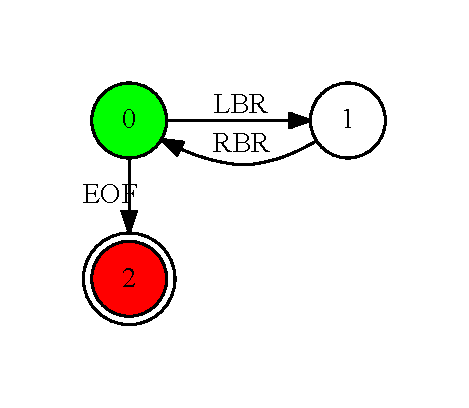
\includegraphics[]{pics/input.pdf}
 \caption{Конечный автомат, задающий регулярную аппроксимацию выражения \textbf{\texttt{expr}}}
 \label{input}
\end{figure}

В результате работы предложенного алгоритма будет получено конечное представление леса разбора SPPF, изображённое на рисунке~\ref{sppf}.

\begin{figure}[!h]
 \centering
 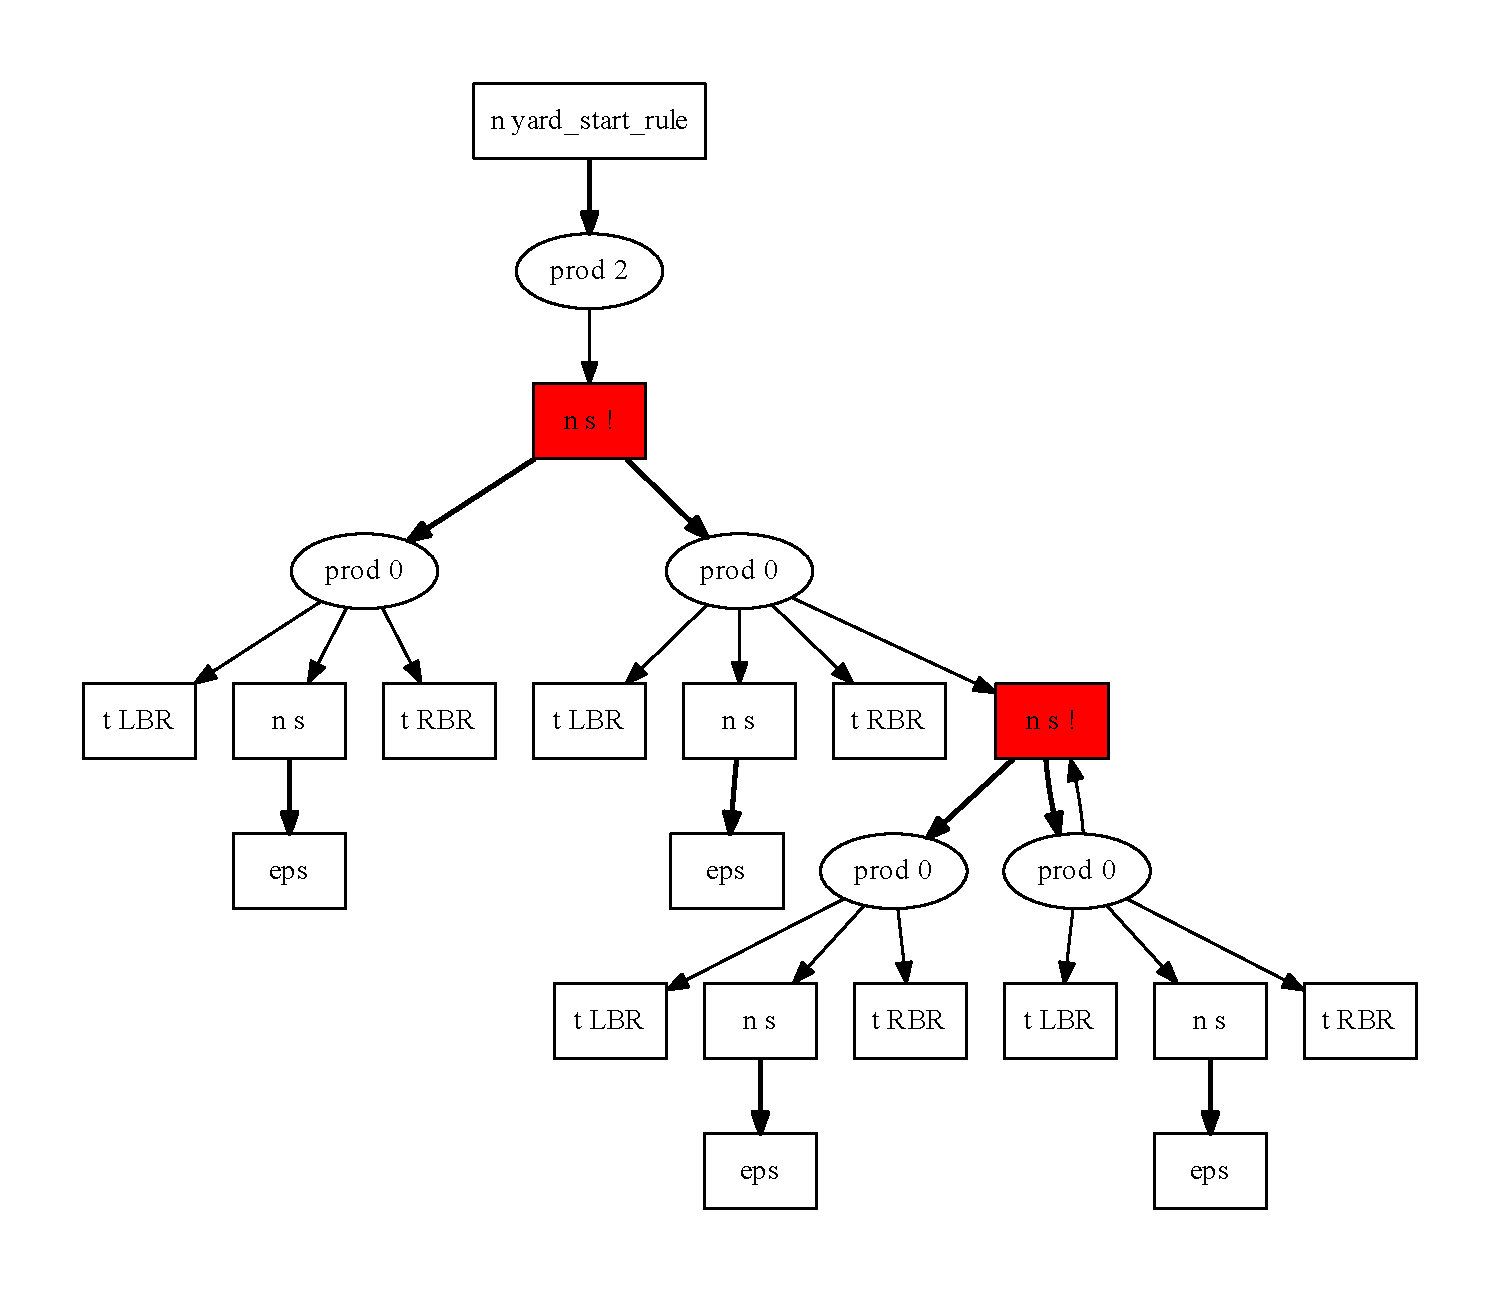
\includegraphics[width=15cm]{pics/sppf.pdf}
 \caption{Конечное представление леса разбора для выражения \textbf{\texttt{expr}}}
 \label{sppf}
\end{figure}

\begin{figure}[!h]
 \centering
 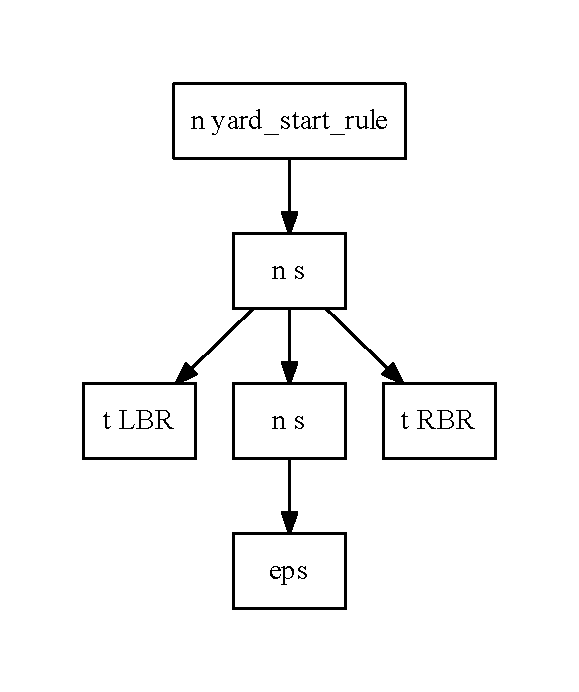
\includegraphics[width=.4\textwidth]{pics/sppf1.pdf}
 \caption{Дерево вывода для выражения $expr="()"$}
 \label{sppf1}
\end{figure}

\begin{figure}[!h]
 \centering
 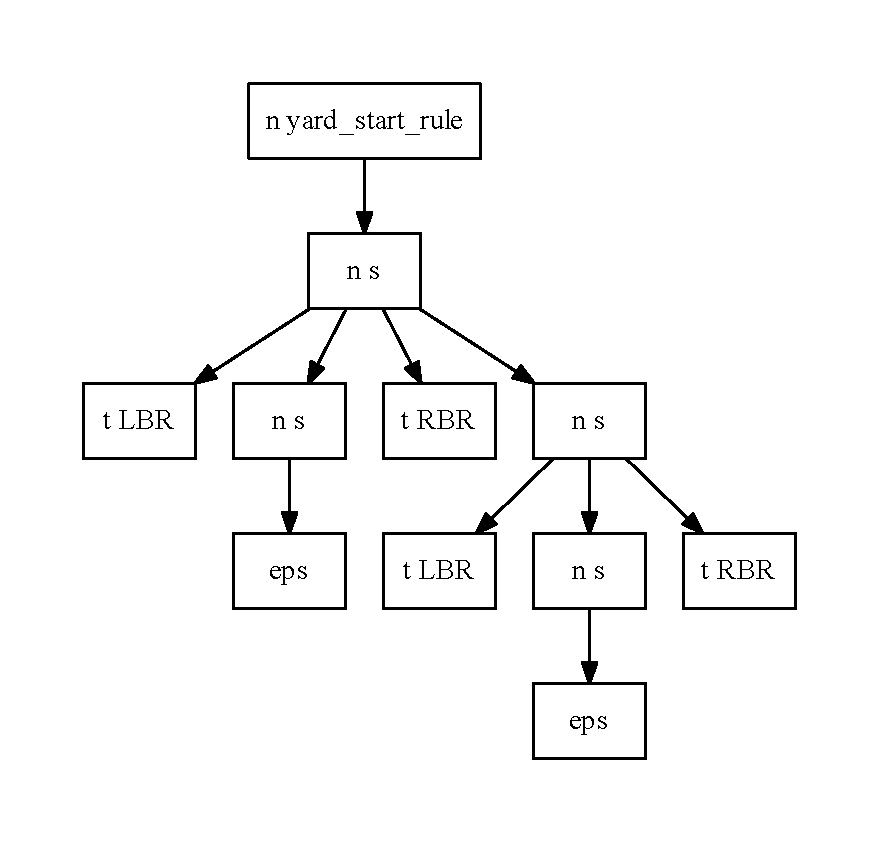
\includegraphics[width=.5\textwidth]{pics/sppf2.pdf}
 \caption{Дерево вывода для выражения $expr="()()"$}
 \label{sppf2}
\end{figure}

\begin{figure}[!h]
 \centering
 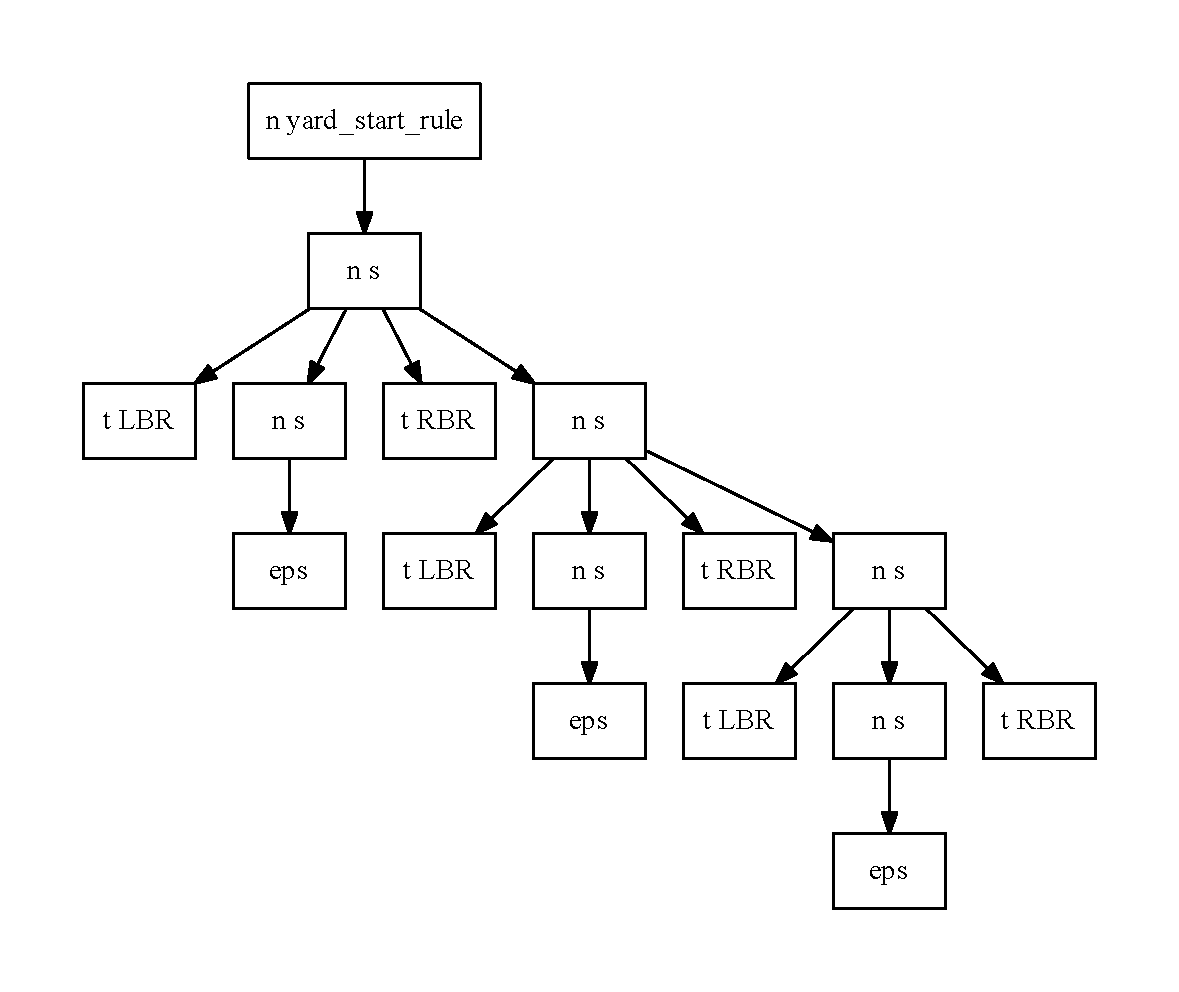
\includegraphics[width=.7\textwidth]{pics/sppf3.pdf}
 \caption{Дерево вывода для выражения $expr="()()()"$}
 \label{sppf3}
\end{figure}

Из построенного SPPF можно извлечь бесконечное количество деревьев, каждое из которых является деревом вывода некоторой цепочки из регулярной аппроксимации. На серии рисунков~\ref{sppf1},~\ref{sppf2},~\ref{sppf3} представлены извлечённые деревья разбора для различных значений выражения \textbf{\texttt{expr}}.  


\section{Доказательство корректности алгоритма ослабленного синтаксического анализа регулярной аппроксимации}

\textsc{Теорема 1.} 
\textit{Алгоритм завершает работу для любых входных данных.}

\textsc{Доказательство.}
С каждой вершиной внутреннего представления графа входного конечного автомата ассоциировано не более $N$ вершин графа GSS, где $N$~--- это количество состояний синтаксического анализатора. Таким образом, количество вершин в графе GSS ограничено сверху числом $N \times n$, где $n$~--- это количество вершин графа входного автомата. Так как в GSS нет кратных ребер, количество его ребер~--- $O((N \times n)^{2})$. На каждой итерации основного цикла алгоритм извлекает из очереди $Q$ и обрабатывает одну вершину внутреннего графа. Вершины добавляются в очередь $Q$ только тогда, когда происходит добавление нового ребра в GSS. Так как количество ребер в GSS конечно, алгоритм завершает работу для любых входных данных. $\square$

Для того, чтобы доказать корректность построения конечного представления леса разбора, нам потребуется следующее определение. 

\textsc{Определение 1.} 
\emph{Корректное дерево}~--- это упорядоченное дерево со следующими свойствами.
\begin{enumerate}
  \item Корень дерева соответствует стартовому нетерминалу грамматики $G$.
  \item Листья соответствуют терминалам грамматики $G$. Упорядоченная последовательность листьев соответствует некоторому пути во входном графе.
  \item Внутренние узлы соответствуют нетерминалам грамматики $G$. Дети внутреннего узла (для нетерминала $N$) соответствуют символам правой части некоторой продукции для $N$ в грамматике $G$.
\end{enumerate}

Таким образом, корректное дерево~--- это дерево вывода некоторой цепочки из регулярного множества в эталонной грамматике. Далее нам необходимо доказать, во-первых, что конечное представление леса разбора SPPF содержит только корректные деревья, во-вторых, что для каждой корректной относительно эталонной грамматики цепочки существует корректное дерево вывода в SPPF. 

\textsc{Лемма.}
\textit{Пусть обрабатывается внутренний граф $\mathcal{G}=(V,E)$. Тогда для каждого ребра GSS $(v_{t}, v_{h})$ такого, что $v_{t} \in V_{t}.processed$, $v_{h} \in V_{h}.processed$, где $V_{t} \in V$ и $V_{h} \in V$, терминалы ассоциированного поддерева соответствуют некоторому пути из вершины $V_{h}$ в $V_{t}$ в графе $\mathcal{G}$.}

\textsc{Доказательство.}
Будем строить доказательство при помощи индукции по высоте дерева вывода $H$. 

База индукции: $H=1$. Возможны два случая.
\begin{enumerate}
  \item Дерево является $\varepsilon$-деревом. Такое дерево соответствует пути длины $0$; начальная и конечная вершины ребра, соответствующего такому дереву, совпадают, поэтому утверждение верно.
  \item Дерево, состоящее из единственной вершины-терминала. Такое дерево соответствует терминалу, считанному с некоторого ребра $(V_{h}, V_{t})$ внутреннего графа, поэтому утверждение верно. 
\end{enumerate}  

Индукционный переход. Пусть корнем дерева высоты $k$ является нетерминал $N$. По третьему пункту определения корректного дерева существует правило эталонной грамматики $N \rightarrow A_{0}, A_{1}, \dots, A_{n}$, где $A_{0}, A_{1}, \dots, A_{n}$ являются детьми корневого узла. Поддерево $A_{i}$ связано с ребром $(v_{t}^{i}, v_{h}^{i})$ графа GSS и, так как его высота не больше $k-1$, то по индукционному предположению существует путь во внутреннем графе из вершины $V_{h}^{i}$ в вершину $V_{t}^{i}$. Вершина $V_{t}^{i} = V_{h}^{i+1}$, так как $v_{t}^{i} = v_{h}^{i+1}$, поэтому во внутреннем графе существует путь из вершины $V_{h}^{0}$ в вершину $V_{t}^{n}$, соответствующий рассматриваемому корректному дереву. $\square$

Так как SPPF является сжатым представлением леса разбора, то для получения конкретного дерева его необходимо \textit{извлечь} из SPPF.

\textsc{Теорема 2.} 
\textit{Любое дерево, извлечённое из SPPF, является корректным.}

\textsc{Доказательство.}
Рассмотрим произвольное дерево, извлечённое из SPPF, и докажем, что оно удовлетворяет определению 1. Первый и третий пункт определения корректного дерева следует из определения SPPF. Второй пункт определения следует из \textsc{леммы}, если применить её к рёбрам из GSS, начало которых лежит на последнем уровне стека и помечено принимающим состоянием, а конец~--- в вершинах на уровне 0. $\square$

\textsc{Теорема 3.} 
\textit{Для каждой строки, соответствующей пути $p$ во входном графе, и выводимой в эталонной грамматике $G$, из SPPF может быть извлечено корректное дерево $t$. То есть $t$ будет являться деревом вывода цепочки, соответствующей пути $p$, в грамматике $G$.}

\textsc{Доказательство.}
Рассмотрим произвольное корректное дерево и докажем, что оно может быть извлечено из SPPF. Доказательство повторяет доказательство корректности для RNGLR-алгоритма~\cite{RNGLR}, за исключением следующей ситуации. RNGLR-алгоритм строит граф GSS по слоям: гарантируется, что $\forall j \in [0..i-1], j-$ый уровень GSS будет зафиксирован на момент построения $i-$ого уровня. В нашем случае это свойство не верно, так как во входном графе могут быть циклы и нет возможности упорядочить обработку его вершин. Это, в свою очередь, может приводить к появлению новых путей для свёрток, которые уже были ранее обработаны. Единственный возможный способ образования такого нового пути~--- это добавление ребра $(v_{t}, v_{h})$, где вершина $v_{t}$ ранее присутствовала в GSS и имела входящие ребра. Так как алгоритм сохраняет информацию о том, какие свёртки проходили через вершины GSS, то достаточно продолжить свёртки, проходящие через вершину $v_{t}$. Таким образом гарантируется выполнение всех возможных свёрток и построение корректного дерева вывода. $\square$

\textsc{Замечание.} Построение леса разбора осуществляется одновременно с построением GSS, при этом дерево вывода нетерминала связывается с ребром GSS каждый раз при обработке соответствующей свёртки, вне зависимости от того, было ли ребро в графе до этого или добавлено на данном шаге. Это обстоятельство позволяет утверждать, что если все возможные редукции были выполнены, то и лес разбора содержит все деревья для всех корректных цепочек из аппроксимации.
